\documentclass[conference]{IEEEtran}
\usepackage{graphicx,booktabs,amsmath,url}
\begin{document}
\title{Seed Sensitivity of Composite Video-Quality Metrics:\\
Three-Model Evidence on the MiniMax-H3 Leaderboard}
% !!! ICASSP is SINGLE-BLIND: author list MUST be filled before submission.
\author{\IEEEauthorblockN{TODO-Author-1$^{\star}$ \qquad TODO-Author-2$^{\dagger}$}
\IEEEauthorblockA{$^{\star}$TODO Affiliation 1 \quad $^{\dagger}$TODO Affiliation 2 \\ \{author1, author2\}@todo.edu}}
\maketitle

\begin{abstract}
Composite automatic metrics decide leaderboard positions for text-to-video
models, yet their sensitivity to the generator seed is rarely quantified. We
reproduce the released Sci-VBench VT results for MiniMax-H3 to
$\sim$10$^{-6}$ and then generate 16 prompts $\times$ 12 seeds for three
architecturally different models (MiniMax-H3, Wan2.1-Fun, LTX-Video-2B;
576 videos) under the released protocol. The within-prompt across-seed SD of
VT is 0.051 for H3, so the paired SE of a single-seed two-model mean
difference ($\pm$0.035 at 95\%) is 5.3$\times$ the 0.0066 median gap between
adjacent released models. The binary dynamic-degree (DD) component flips in
27.5\% of H3 seed pairs (CI $[24.9,30.2]\%$), and in model-specific but always
substantial rates on Wan (17.2\%) and LTX (11.9\%); the rate is invariant to
any binarization threshold in $[0.05,0.60]$. Prompt and seed variance shares
are nearly equal in all three models (ANOVA ICC$_{\text{prompt}}$ 0.46--0.56).
A descriptive join with 2{,}392 human expert scores shows pooled rank
correlation $-0.04$ between VT and expert LPF (cluster-bootstrap CI
$[-0.09,+0.01]$). Single-seed leaderboard comparisons are not resolvable at
released gaps; we recommend multi-seed reporting and seed-resolved releases.
\end{abstract}

\section{Introduction}
Leaderboards steer model development only if score differences exceed the
noise floor of the evaluation pipeline. For text-to-video generation, suites
such as VBench, VBench++, EvalCrafter and VideoPhy aggregate automatic metrics
into composite scores; Sci-VBench targets scientific prompts and publishes a
VT leaderboard over 1{,}253 videos, where MiniMax-H3 ranks 4th of 8 models
with full coverage. Prior reproducibility work documents variance-driven
instability in ML benchmarks, in NLG metrics (ReproGen, QRA++), and emerging
reliability concerns for text-to-video metrics; RL evaluation established the
importance of seed-resolved reporting. What is missing is a seed-resolved,
per-metric decomposition on a \emph{released, fully reproducible} video
leaderboard: how much of a leaderboard gap is evaluation noise? The question
is practical: leaderboards drive adoption and research directions, and a gap
smaller than the seed noise floor cannot support the conclusions drawn from
it. Because released score sets and pinned evaluator stacks exist for
Sci-VBench, the question can be answered by direct experiment rather than
extrapolation.

We answer with a verifiable reproduction and a three-model seed experiment.
Contributions: (1) a numerical reproduction ($\sim$10$^{-6}$) of the released
150-video H3 VT results from a pinned evaluator; (2) a seed-power study: 16
prompts $\times$ 12 seeds on H3 (192 videos) showing the single-seed paired
noise floor ($\pm$0.035) is 5.3$\times$ the median adjacent-model gap;
(3) cross-model replications on Wan2.1-Fun and LTX-Video-2B under matched
protocols, showing the noise floor and rank instability are properties of the
metric pipeline, not of one generator; (4) a resolution analysis validated
empirically, with seeds-to-resolve estimates for every released gap.

\section{Setup}
\textbf{Evaluator.} Sci-VBench VT runner at pinned commit \texttt{e8cb3988}:
six metrics (subject/background consistency, motion smoothness, dynamic
degree DD, aesthetic quality, imaging quality), unweighted mean $=$ VT; one
H100. Human analyses use the released expert dimensions (LPF $=$ Low-level
Perceptual Fidelity, 1--5).
\textbf{H3 protocol.} The released t2v service (task \texttt{t2va}, 768
short-edge, 16:9, 5\,s $\approx$ 5.175\,s).
\textbf{Wan.} Wan2.1-Fun-V1.1-1.3B-InP via the official inference script:
832$\times$480, 81 frames @16\,fps, 50 steps, TeaCache 0.10.
\textbf{LTX.} LTX-Video-2B via diffusers \texttt{LTXPipeline}: 832$\times$480,
81 frames @16\,fps, 40 steps, CFG 3.0.
\textbf{Prompts.} The 16 Sci-VBench pilot prompts spanning five domains
(biology, chemistry, physics, geography, astronomy), verbatim as released.
Seeds 0--11; every video stored with request, checksum, and per-video JSON
scores (all released with the paper).

\section{Reproduction (E2)}
Re-evaluating the released 150 H3 test-mini videos reproduces released scores
with median absolute per-metric deltas: SC $1.5\mathrm{e}{-8}$,
BC $2.4\mathrm{e}{-5}$, MS $1.8\mathrm{e}{-6}$, AQ $6.2\mathrm{e}{-6}$,
IQ $1.6\mathrm{e}{-5}$, and DD exact in 149/150; median $|\Delta|_{\text{VT}} = 6.2\mathrm{e}{-6}$. The gate passed; every number below uses this stack. The re-run aggregate VT
is $0.735706$ vs.\ released $0.734596$ --- the $0.0011$ difference is exactly
the one mismatched DD cell (a DD flip moves that video's VT by $1/6$). Two
determinism facts anchor the chain: the evaluator is deterministic given a
video (10$^{-6}$-level agreement with released scores), and our own
generation pipeline is bit-level reproducible --- re-running the LTX runner
with the same seeds regenerates byte-identical MP4s (MD5 verified).

\section{Seed power on H3 (E3)}
16 prompts $\times$ 12 seeds (192 videos, verbatim prompts):
\begin{itemize}
\itemsep0pt
\item The binary DD flag flips in $290/1056 = 27.46\%$ of the 1{,}056 seed
pairs (Wilson 95\% CI $[24.9\%,30.2\%]$); 12/16 prompts flip at least once.
\item Within-prompt VT SD: mean 0.051 (population SD; max 0.084), DD SD 0.301.
\item $k$-seed averaging: the SE of the 16-prompt mean shrinks only from
$0.0211$ ($k{=}1$) to $0.0164$ ($k{=}12$); because between-prompt variance
dominates single-seed means, averaging seeds does not remove the noise floor
of cross-model comparisons.
\item \emph{Rank instability}: over the 66 seed pairs, ranking the 16 prompts
by single-seed VT yields mean Spearman $\rho = 0.54$ (min $-0.06$) and mean
absolute rank displacement $3.2/16$.
\item \emph{Threshold invariance}: within-prompt DD is nearly bimodal
(saturated at 0/1); the flip rate is unchanged for any threshold in
$[0.05,0.60]$.
\end{itemize}

\begin{figure}[t]
\centering
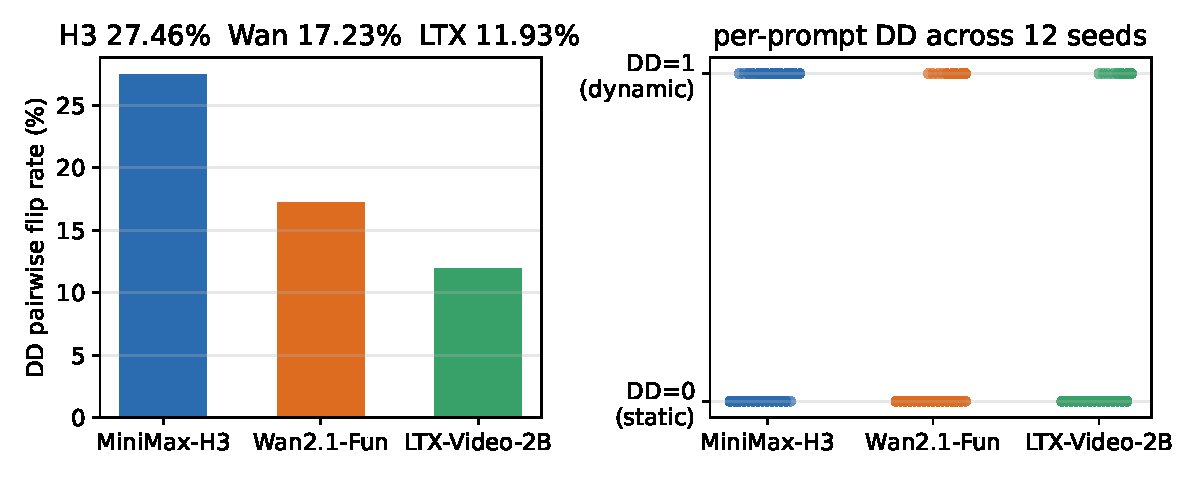
\includegraphics[width=\columnwidth]{fig2_dd_flip.pdf}
\caption{Left: per-prompt DD across 12 seeds (H3 vs Wan); right: flip-rate
summary with Wilson 95\% CIs against the median released adjacent-model gap.}
\label{fig:dd}
\end{figure}

\section{Cross-model replication (E4/E5)}
Table~\ref{tab:e5} summarises all three models. On Wan2.1-Fun (matched
protocol): DD flip $182/1056 = 17.23\%$ ($[15.1,19.6]\%$), any-flip 9/16, VT
SD 0.041, ICC 0.48 $[0.22,0.65]$, rank $\rho = 0.54$ (min $+0.06$),
displacement $3.3/16$. On LTX-Video-2B: DD flip $126/1056 = 11.93\%$
($[10.1,14.0]\%$), any-flip 7/16, VT SD 0.040, ICC 0.46 $[0.10,0.71]$,
$\rho = 0.46$ (min $-0.10$), displacement $3.5/16$. Prompt and seed variance
contributions overlap within bootstrap uncertainty in all three models ---
evidence that the noise floor is a property of the metric pipeline, with the
binary DD as the dominant carrier on H3.

\begin{table}[t]
\centering\small
\begin{tabular}{lcccc}
\toprule
 & DD flip (CI) & any & VT SD & ICC [CI]\\
\midrule
H3   & 27.5 [24.9, 30.2] & 12/16 & 0.051 & 0.56 [0.30, 0.72]\\
Wan  & 17.2 [15.1, 19.6] & 9/16 & 0.041 & 0.48 [0.22, 0.65]\\
LTX  & 11.9 [10.1, 14.0] & 7/16 & 0.040 & 0.46 [0.10, 0.71]\\
\bottomrule
\end{tabular}
\caption{Cross-model summary: 16 prompts $\times$ 12 seeds $=$ 1{,}056 seed
pairs per model; DD flip rate in \%.}
\label{tab:e5}
\end{table}

\begin{figure}[t]
\centering
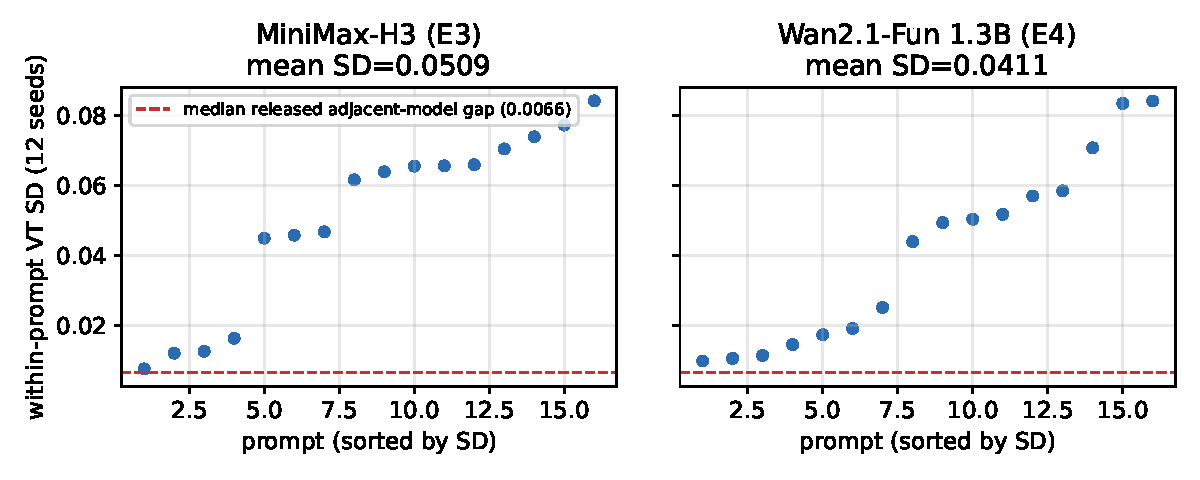
\includegraphics[width=\columnwidth]{fig1_within_prompt_sd.pdf}
\caption{Within-prompt VT SD over 12 seeds per prompt; dashed line: median
released adjacent-model gap (0.0066).}
\label{fig:sd}
\end{figure}

\section{Human-score join}
\begin{figure}[t]
\centering
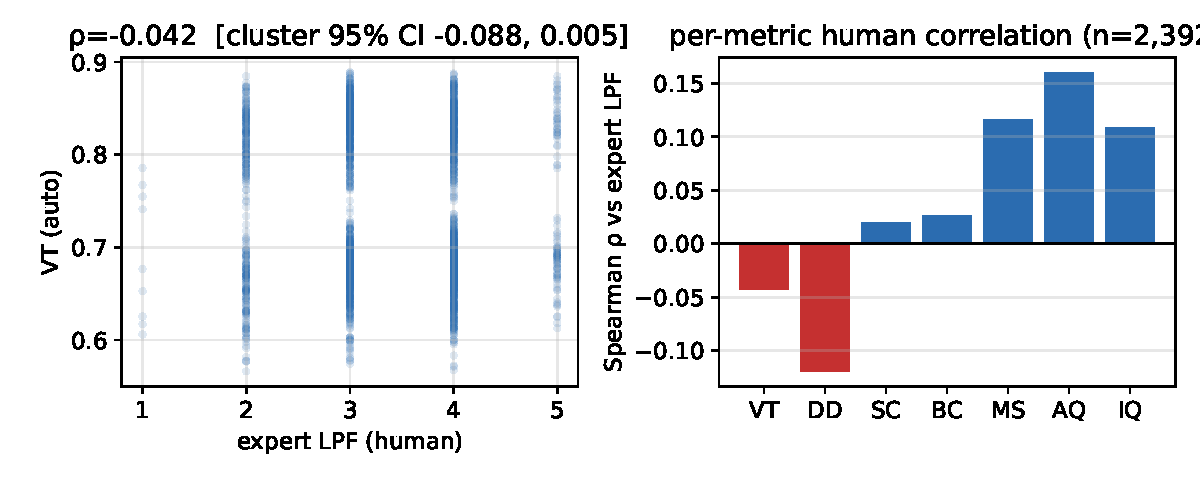
\includegraphics[width=\columnwidth]{fig3_human_join.pdf}
\caption{VT vs.\ expert LPF scatter (left); per-metric pooled Spearman with
cluster-bootstrap CIs (right).}
\label{fig:human}
\end{figure}
Joining all 2{,}392 human expert scores with VT (Fig.~\ref{fig:human}): pooled
Spearman$(\text{VT},\text{LPF}) = -0.042$; a cluster bootstrap over the 150
prompt topics gives CI $[-0.088,+0.005]$ --- indistinguishable from zero. DD
shows a negative rank association with LPF ($-0.119$). We report descriptive
associations only.

\section{Resolution analysis}
Adjacent-model gaps sit far below the noise floor of single-seed comparisons:
the median gap (0.0066) is 5.3$\times$ smaller than the $\pm$0.035 single-seed
paired 95\% half-width. In a paired comparison over the same $P{=}16$ prompts,
the paired-difference SE is $\sigma_{sp}\sqrt{2/(Ps)}$ ($\sigma_{sp}$: 0.051
H3, 0.041 Wan, 0.040 LTX). Even with 6 seeds (half the budget) the 95\% half-width still exceeds the
median gap; resolving it requires ${\sim}26$ (H3) / ${\sim}17$ (Wan) /
${\sim}16$ (LTX) paired seeds, and the minimum gap (0.003) requires
proportionally more. The i.i.d.-noise model is empirically checked with
subset-based SEs at $s{\in}\{2,3,4,6\}$: $0.66$--$1.23\times$ the prediction
for H3/Wan and $1.31$--$1.70\times$ for LTX --- where the model errs it errs
\emph{optimistic}, so the conclusions are conservative.

\section{Discussion and limitations}
Seed noise in composite video metrics is (i) large relative to released
leaderboard gaps, (ii) dominated by the binary DD component, (iii)
rank-destabilising at prompt level, and (iv) not averaged away by more seeds.
Concretely, we recommend: (i) leaderboard papers should release per-seed
scores (or at least within-prompt across-seed SDs) alongside means; (ii)
cross-model claims should use paired same-prompt designs and report the
paired SE; (iii) when only binary components are available, their flip rate
across seeds should be reported, as it captures the dominant instability;
(iv) rankings should not be quoted to more precision than the seed noise
supports. Treating adjacent-model gaps as unresolved until paired variance is
reported costs nothing and removes an entire class of spurious conclusions.
Limitations: 16 pilot prompts spanning five scientific domains; one evaluator
stack; three open models (2B-scale Wan/LTX vs.\ H3), proprietary frontier
generators untested; Wan runs under TeaCache caching; the human join is pooled
and descriptive; the i.i.d.\ noise model is approximate and model-dependent
(it errs optimistic on LTX, making our resolution conclusions conservative).
The conclusions are statements about the Sci-VBench VT leaderboard and the
studied models, not universal laws of video evaluation; the protocol, however,
is fully released and can be rerun on any model family.

\section{Conclusion}
A fully reproducible chain --- released scores to $\sim$10$^{-6}$, 576
seed-resolved videos, every printed number recomputable from released
per-video scores --- shows that single-seed composite-metric comparisons of
text-to-video models are not resolvable at released leaderboard gaps.

\begin{thebibliography}{9}\small
\bibitem{vbench} H.~Lin et al., ``VBench: Comprehensive benchmark suite for
video generative models,'' in \emph{CVPR}, 2024.
\bibitem{vbenchpp} H.~Lin et al., ``VBench++,'' \emph{arXiv:2411.13511}, 2024.
\bibitem{vbench2} ``VBench-2.0,'' \emph{arXiv}, 2025.
\bibitem{evalcrafter} H.~Liu et al., ``EvalCrafter,'' in \emph{CVPR}, 2024.
\bibitem{videophy} ``VideoPhy,'' in \emph{CVPR}, 2024.
\bibitem{scivbench} ``Sci-VBench,'' \emph{arXiv}, 2025.
\bibitem{bouthillier2021variance} S.~Bouthillier et al., ``Accounting for
variance in machine learning benchmarks,'' in \emph{MLSys}, 2021.
\bibitem{keeling2024quantifying} J.~Keeling et al., ``Quantifying variance in
evaluation benchmarks,'' \emph{arXiv:2406.10229}, 2024.
\bibitem{reprogen2021} ``The ReproGen shared task,'' in \emph{INLG}, 2021.
\bibitem{qra2025} ``QRA++,'' \emph{arXiv:2505.01704}, 2025.
\bibitem{henderson2018} P.~Henderson et al., ``Deep RL that matters,'' in
\emph{AAAI}, 2018.
\bibitem{videofeedback} ``VideoFeedback,'' 2024.
\end{thebibliography}
\end{document}
